\documentclass{article} % For LaTeX2e
\usepackage{nips14submit_e,times}
\usepackage{amsmath}
\usepackage{amsthm}
\usepackage{amssymb}
\usepackage{mathtools}
\usepackage{hyperref}
\usepackage{url}
\usepackage{algorithm}
\usepackage[noend]{algpseudocode}
%\documentstyle[nips14submit_09,times,art10]{article} % For LaTeX 2.09

\usepackage{graphicx}
\usepackage{caption}
\usepackage{subcaption}

\def\eQb#1\eQe{\begin{eqnarray*}#1\end{eqnarray*}}
\def\eQnb#1\eQne{\begin{eqnarray}#1\end{eqnarray}}
\providecommand{\e}[1]{\ensuremath{\times 10^{#1}}}
\providecommand{\pb}[0]{\pagebreak}
\DeclarePairedDelimiter\ceil{\lceil}{\rceil}
\DeclarePairedDelimiter\floor{\lfloor}{\rfloor}

\newcommand{\E}{\mathrm{E}}
\newcommand{\Var}{\mathrm{Var}}
\newcommand{\Cov}{\mathrm{Cov}}

\def\Qb#1\Qe{\begin{question}#1\end{question}}
\def\Sb#1\Se{\begin{solution}#1\end{solution}}

\newenvironment{claim}[1]{\par\noindent\underline{Claim:}\space#1}{}
\newtheoremstyle{quest}{\topsep}{\topsep}{}{}{\bfseries}{}{ }{\thmname{#1}\thmnote{ #3}.}
\theoremstyle{quest}
\newtheorem*{definition}{Definition}
\newtheorem*{theorem}{Theorem}
\newtheorem*{lemma}{Lemma}
\newtheorem*{question}{Question}
\newtheorem*{preposition}{Preposition}
\newtheorem*{exercise}{Exercise}
\newtheorem*{challengeproblem}{Challenge Problem}
\newtheorem*{solution}{Solution}
\newtheorem*{remark}{Remark}
\usepackage{verbatimbox}
\usepackage{listings}
\usepackage{mathrsfs}
\title{Functional Analysis: \\
Problem Set II}


\author{
Youngduck Choi \\
CIMS \\
New York University\\
\texttt{yc1104@nyu.edu} \\
}


% The \author macro works with any number of authors. There are two commands
% used to separate the names and addresses of multiple authors: \And and \AND.
%
% Using \And between authors leaves it to \LaTeX{} to determine where to break
% the lines. Using \AND forces a linebreak at that point. So, if \LaTeX{}
% puts 3 of 4 authors names on the first line, and the last on the second
% line, try using \AND instead of \And before the third author name.

\newcommand{\fix}{\marginpar{FIX}}
\newcommand{\new}{\marginpar{NEW}}

\nipsfinalcopy % Uncomment for camera-ready version

\begin{document}


\maketitle

\begin{abstract}
This work contains solutions to the exercises of the problem set II.
\end{abstract}

\bigskip

\begin{question}[1]
\hfill
\begin{figure}[h!]
  \centering
    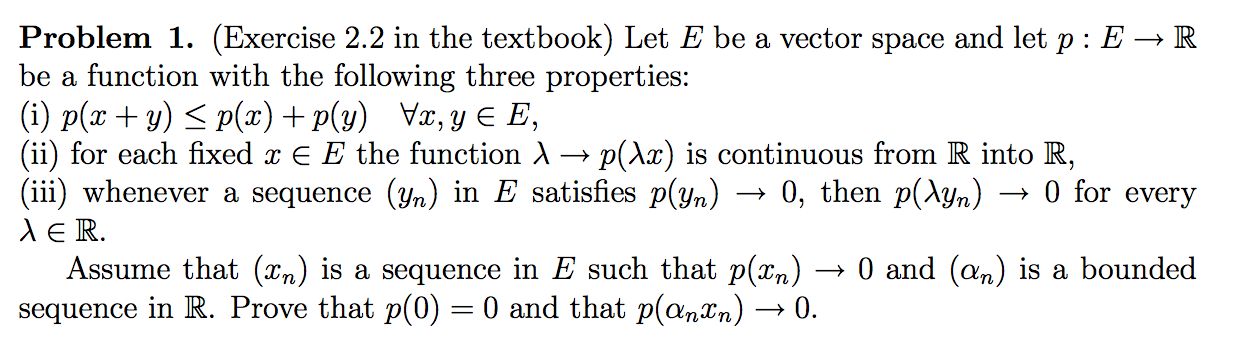
\includegraphics[width=0.7\textwidth]{funcA-h-e2-p1.png}
\end{figure}
\end{question}
\begin{solution} \hfill \\
Fix $\epsilon > 0$. Suppose for sake contradiction that there exists
a subsequence $\{a_{n_k} x_{n_k}\}$ such that 
\eQb
|p(a_{n_k}x_{n_k})| \geq 2\epsilon \>\>\> (*)
\eQe
for all $k \geq 1$
Since $\{a_n\}$ is bounded, 
passing to a further subsequence, and relabeling, we may suppose that
\eQb
|p(a_{n} x_{n}) | \geq 2\epsilon &\text{and}& \lim_{n \to \infty} a_n = a
\eQe
for any $n \geq 1$ and for some $a \in \mathbb{R}$. 
Now, observe that $\phi_k:\mathbb{R} \to \mathbb{R}$ defined by 
\eQb
\lambda &\mapsto& |p(\lambda x_k)| \>\>\> (\lambda \in \mathbb{R})
\eQe
for each $k \geq 1$ is continuous by (ii). Therefore,  
\eQb
F_n &=& \bigcap_{k=n}^{\infty} {\phi_k}^{-1}([-\epsilon,\epsilon])
\eQe
is closed for each $n \geq 1$ ($F_n$ given in the hint). 
By assumption and (iii), it follows that
\eQb
\bigcup_{n} F_n &=& \mathbb{R}
\eQe 
and by Baire-Category, we can choose $n_0 \in \mathbb{N}$ such that there
exists $\lambda_0 \in \mathbb{R}$ and $\delta > 0$ such that 
\eQb
B(\lambda_0,\delta) \subset F_{n_0}.
\eQe
Now, by (i), we obtain
\eQb
p(a_k x_k) &\leq& p((\lambda_0 + a_k - a) x_k) + p((a - \lambda_0) x_k) 
\eQe
and
\eQb
-p(a_k x_k) &\leq& -p((\lambda_0 + a_k - a) x_k) + p((\lambda_0 - a)x_k)
\eQe
for each $k \geq 1$. Now for all $k$ large enough, since $(a - \lambda_0), 
(\lambda_0 - a)$
are fixed constants, we have
\eQb
(\lambda_0 + a_k - a) \in B(\lambda_0,\delta) \>\>\> \text{and} \>\>\> 
|p((a- \lambda_0)|,|p(\lambda_0 - a)| < \epsilon
\eQe
so
\eQb
|p(a_k x_k)| &<& 2\epsilon,
\eQe
which contradicts $(*)$.  



\end{solution}

\newpage

\begin{question}[2]
\hfill
\begin{figure}[h!]
  \centering
    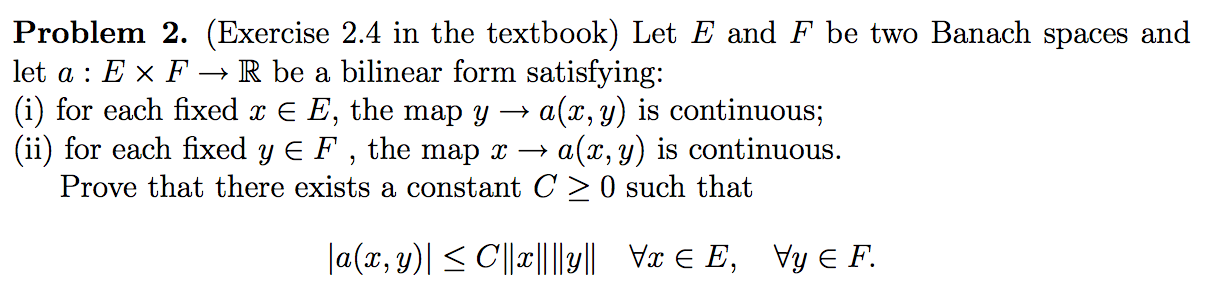
\includegraphics[width=0.7\textwidth]{funcA-h-e2-p2.png}
\end{figure}
\end{question}
\begin{solution} \hfill \\
\end{solution}

\newpage

\begin{question}[3]
\hfill
\begin{figure}[h!]
  \centering
    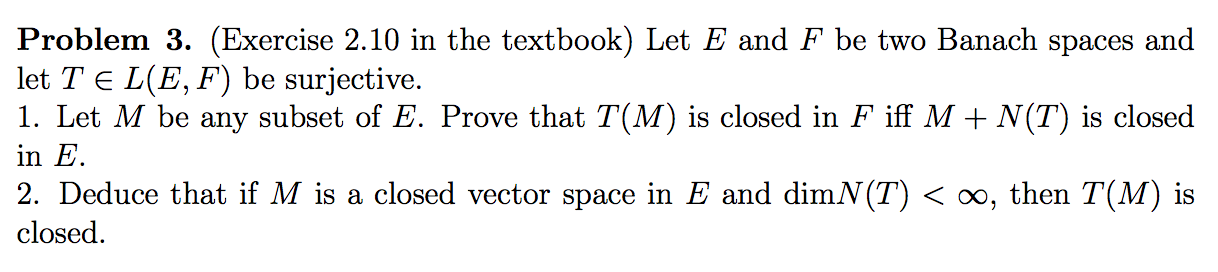
\includegraphics[width=0.7\textwidth]{funcA-h-e2-p3.png}
\end{figure}
\end{question}
\begin{solution} \hfill \\
\end{solution}

\newpage

\begin{question}[4]
\hfill
\begin{figure}[h!]
  \centering
    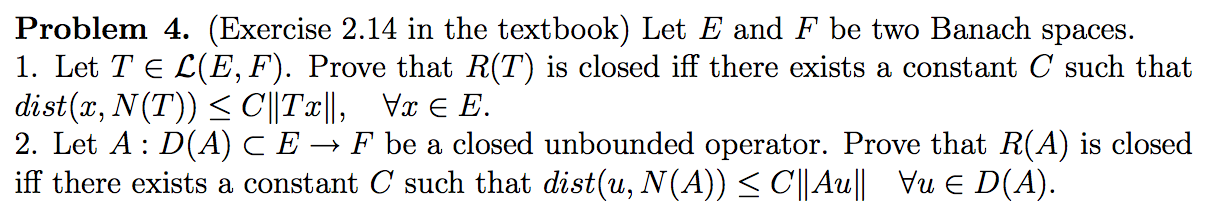
\includegraphics[width=0.7\textwidth]{funcA-h-e2-p4.png}
\end{figure}
\end{question}
\begin{solution} \hfill \\
\end{solution}

\newpage

\begin{question}[5]
\hfill
\begin{figure}[h!]
  \centering
    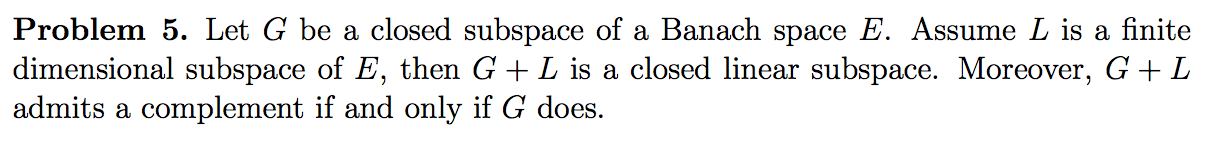
\includegraphics[width=0.7\textwidth]{funcA-h-e2-p5.png}
\end{figure}
\end{question}
\begin{solution} \hfill \\
\end{solution}

\newpage

\begin{question}[6]
\hfill
\begin{figure}[h!]
  \centering
    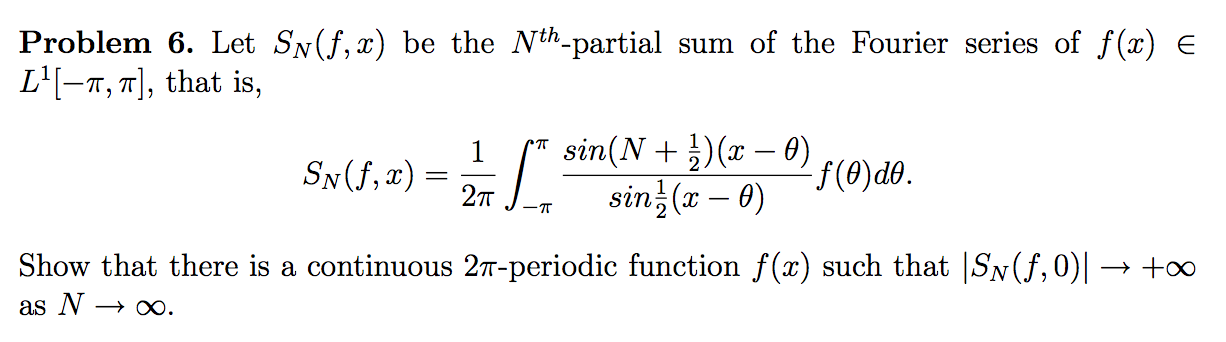
\includegraphics[width=0.7\textwidth]{funcA-h-e2-p6.png}
\end{figure}
\end{question}
\begin{solution} \hfill \\
\end{solution}

\newpage

\begin{question}[7]
\hfill
\begin{figure}[h!]
  \centering
    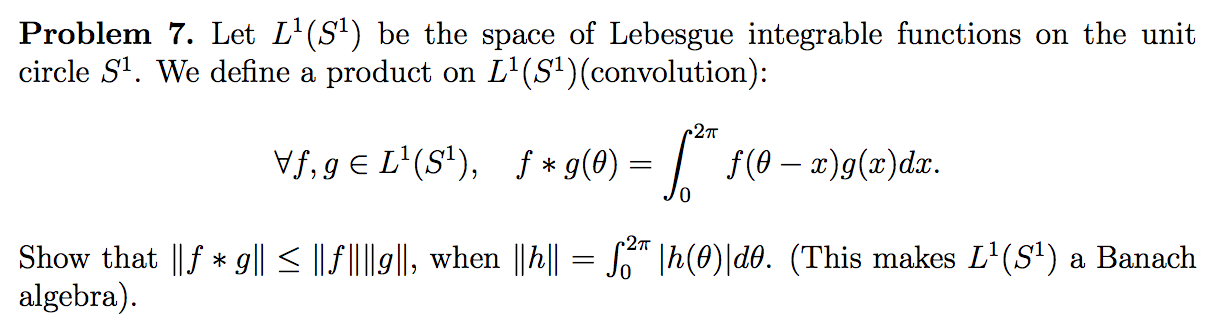
\includegraphics[width=0.7\textwidth]{funcA-h-e2-p7.png}
\end{figure}
\end{question}
\begin{solution} \hfill \\
By Tonelli's theorem and the translation invariance property of Lebesgue measure,
\eQb
||f * g|| &=& \int_{0}^{2\pi} |\int_{0}^{2\pi} f(t - x)g(x) dx | dt  
\leq  \int_{0}^{2\pi}\int_{0}^{2\pi} |f(t-x)g(x)| dx dt \\
&=& \int_{0}^{2\pi} \int_{0}^{2\pi} |f(t-x)g(x)| dt dx 
= \int_{0}^{2\pi} |g(x)| \int_{0}^{2\pi} |f(t-x)| dt dx \\
&=& ||f|| \int_{0}^{2\pi} |g(x)| = ||f|| ||g|| 
\eQe
for any $f,g \in L^1(S^1)$. \hfill $\qed$ 


\end{solution}

\newpage

\begin{question}[8]
\hfill
\begin{figure}[h!]
  \centering
    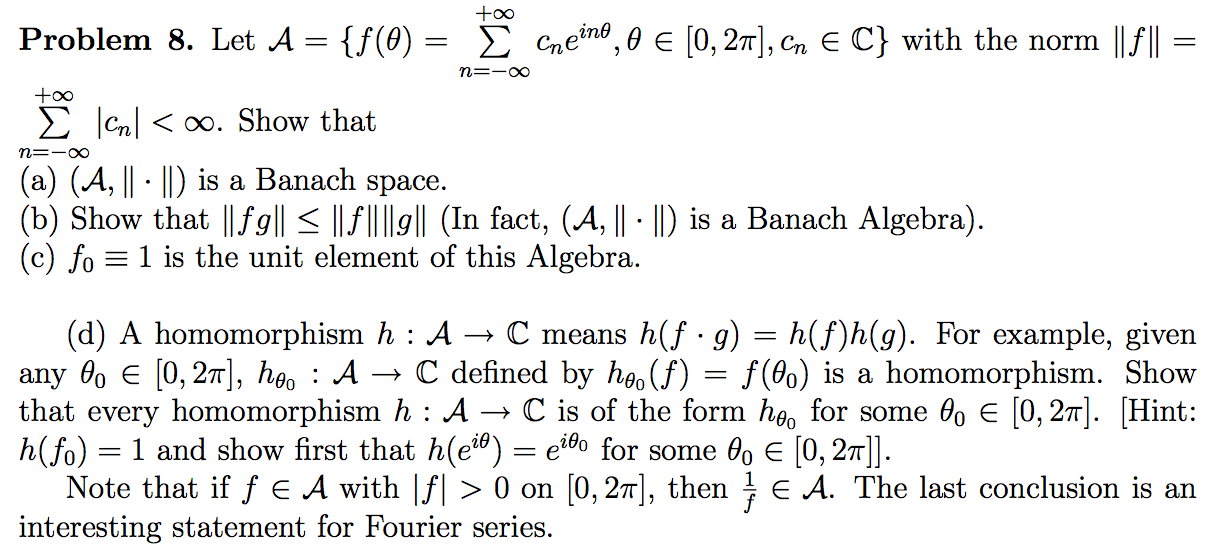
\includegraphics[width=0.7\textwidth]{funcA-h-e2-p8.png}
\end{figure}
\end{question}
\begin{solution} \hfill \\
\end{solution}





\end{document}
